Como ya se ha mencionado, este dispositivo es un prototipo. La forma de proceder de \textit{Tritium}, y en general de un experimento, es realizar todas las medidas posibles sobre éste y, cuando ya no podamos obtener más información, fabricar un nuevo prototipo que supere las limitaciones encontradas en el anterior. Nuevamente, realizar la misma labor sobre el siguiente prototipo. Se considerará que se ha llegado al diseño final cuando hayamos llegado al objetivo final del proyecto \textit{Tritium} (detectar actividades del orden de cientos de $\becquerel/L$) o ya no podamos aplicar mejoras para conseguir una optimización del sistema de detección y poder, de esta forma, detectar niveles de actividades más bajas.

Según se ha calculado  en la seccion $\ref{sec:Resultados}$, nuestro dispositivo presenta una actividad aproximada de $108.11~\mega\becquerel/\liter$. Podemos observar que todavía estamos lejos del límite actual~\cite{Rat}, por lo que, según se ha explicado, el siguiente paso es pasar a diseñar una nueva versión del prototipo. 

Hay que tener en cuenta que aún podemos realizar una serie de medidas sobre este prototipo, tales como el cálculo de su eficiencia de fotodetección, los cuales nos permitirá determinar otras posibles mejoras que serán implementadas en el siguiente prototipo. Es importante obtener el máximo de información de cada prototipo para poder incluir una mayor optimización en la siguiente versión y, de esta forma, necesitar un menor número de prototipos para llegar al diseño final (abaratando de esta forma el proceso de I+D). 

A pesar de que todavía se realizarán más medidas sobre este prototipo, ya se han encontrado ciertas limitaciones que serán subsanadas  en la siguiente versión. Estas se citan a continuación:
\begin{enumerate}
\item{} En primer paso será la realización de medida con los SiPM con los que se realizó la calibración (Sec~$\ref{sec:SiPM}$) ya que en el prototipo utilizado hasta el momento únicamente se han empleado PMT. El punto más importante de la sustitución de los PMTs por los SiPMs será la obtención de una mayor eficiencia del sistema, ya que los PMTs poseen una eficiencia bastante inferior, $30\%$, en comparación con los SiPMs, $50\%$.

Para poder depositar de forma segura los SiPM sobre el prototipo sera necesario el diseño de nuevas piezas de sujeción, ya que las actuales (Fig. $\ref{tapones}$) estaban específicamente diseñadas para la sujeción de los PMT.

\item{} Hay que tener en cuenta que se utilizaron los SiPM modelo S13360-1375CS de Hamamatsu Photonics (Sec. $\ref{sec:Equipo}$) de forma provisional, ya que son los que estaban disponibles en el laboratorio de reacciones nucleares y su espectro de PDE cumplía con los requisitios del proyecto (Fig. $\ref{Espectros}$). Además son de tipo CS, es decir, disponen de dos terminaciones para una conexión rápida y no permanente. 
Sin embargo, la propuesta final de Tritium sería utilizar fotomultiplicadores modelo S13360-6075PE,  que presentan exactamente las mismas características que los anteriormentne mencionados, pero con un mayor tamaño, con una superficie total activa de $6 \times 6 \mm^2$,  que les permite incluir $6000$ píxeles, lo que  implica un mayor rango dinámico. Además, estos SiPM son de tipo PE, es decir, presentan unas terminaciones que tiene que ir soldadas a la placa por lo que, para su utilización, se necesita disponer de la placa final que se utilizará en el prototipo. 
Dado que estos tienen que ir dispuestos sobre la tarjeta final del prototipo, retrasamos su utilización y, por el momento, realizaremos todas las pruebas sobre los SiPM actualmente utilizados, ya que ambos tienen similares características en casi todos los aspectos.

\item{} En tercer lugar se pretende sustituir la tarjeta conversora (fig. $\ref{TarjetaSiPM}$), tarjeta diseñada para NEXT, por una tarjeta especialmente diseñada para nuestro fin. Antes de empezar a diseñar la nueva tarjeta,  consideraremos todas las características necesarias que deban  ser implementadas  en el siguiente prototipo.
Por un lado, uno de los pilares fundamentales del proyecto \textit{Tritium} será crear un proceso de automatización que compense las variaciones de la ganancia debidas a cambios en la temperatura, compensadas con cambios en el voltaje operacional (Sec. $\ref{sec:Compensacion}$).
Por otro lado, el diseño final del detector que pretende desarrollar el proyecto \textit{Tritium} presenta un gran número de haces de fibras centelleadoras, a priori  desconocido, y que habrá que calcular con ayuda de simulaciones, y, por extensión, necesitaremos un gran número de SiPM en las terminaciones de estos haces. Debido a ello, nos encontramos con la necesidad de desarrollar un proceso automático de calibración de los SiPM.  
Por todo ello, la tarjeta diseñada para el segundo prototipo deberá de ser capaz de llevar a cabo el proceso  de automatización. 
Para empezar con el diseño a pequeña escala de este proceso de automatización, se utilizará una tarjeta que sólo contiene cuatro posibles entradas (cada una de las cuales estará asociada a un SiPM). Además, dispone de varios caminos para realizar esta automatización (por medio de relés o multiplexores) y dispone de la posibilidad de obtener la señal amplificada o sin amplificar, lo que nos permitirá determinar cual de todos estos caminos tiene menos cross-talk entre señales y da mejores resultados. Esta tarjeta  se diseñó en el IFIC para el proyecto NEXT-100, que requiere unos requisitos muy similares a los nuestros~\cite{Marc}. Esta tarjeta puede verse en la figura~\ref{arduino} izquierda.

Habrá que familiarizarse con el programa LabView, programa elegido para desarrollar el código de automatización, ya que cumple con todos los requisitos impuestos por el proyecto, disponemos de trabajos anteriores muy similares a nuestro proyecto realizados con este programa por compañeros del IFIC y, además, el IFIC posee licencia para su uso. También habrá que familiarizarse con el uso de algún tipo de micorcontrolador capaz de realizar esta labor de automatización. En concreto se utilizaran Arduinos, ya que son rápidos, eficaces y económicos. El arduino utilizado, Arduino Mega, puede verse  en la figura~\ref{arduino}  derecha.

\begin{figure}[htb]
\centering
{
%\subfloat[Espectro de emisión]
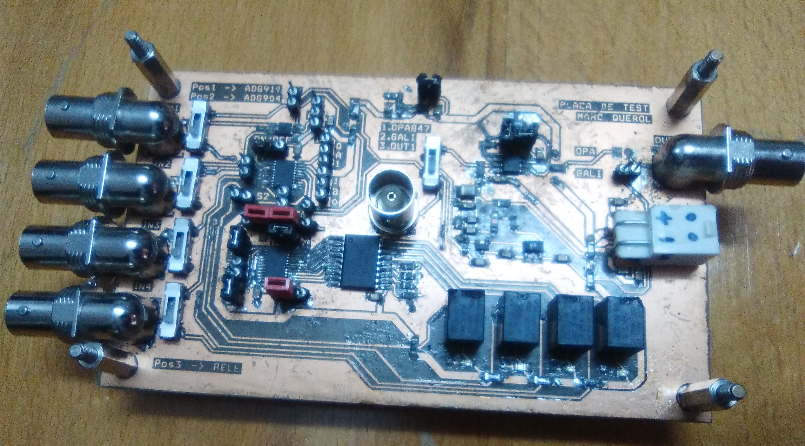
\includegraphics[scale=0.25]{Tarjeta1.png} 
}
{
%\subfloat[Espectro de emisión]
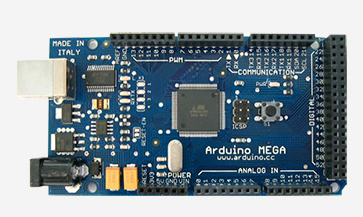
\includegraphics[scale=0.5]{Arduino.png} 
}
\caption{Tarjeta de automatización y Arduino Mega\label{arduino}}
\end{figure} 

Lo más importante de esta tarjeta es que, por un lado, realiza el proceso de automatización y, por otro, nos permite interaccionar con todas las partes importantes de nuestro experimento, tales como fuente de tensión de alimentación,  distintos componentes del sistema, osciloscopios, etc., mediante LabView.
Como ya se ha mencionado anteriormente esta tarjeta formará parte de un prototipo. El diseño final contendrá un número mucho mayor de haces de fibras centelleadoras, necesitando un número elevado de SiPM su lectura. Es de vital importancia  la automatización tanto de la calibración de SiPM como del control de componentes, ya que calibrar un número elevado de SiPM (en principio se han previsto 64 SiPM) es un trabajo que llevaría demasiado tiempo. Además, para poder controlar de forma efectiva un número tan elevado de SiPM, es necesario un control automático. 

\item {} En cuarto lugar, también habrá que proceder a aluminizar las fibras centelleadoras  por evaporación en vacío, proceso que se realizará en el ICMOL, tema discutido en la sección~\ref{sec:Resultados}.

\item {} En quinto lugar, hemos observado que la electrónica empleada presenta una gran cantidad de ruido, por lo que será necesario conseguir electrónica de bajo ruido en un futuro, para poder separar la señal del fondo.

\item {} En sexto lugar, habrá que mejorar las simulaciones, incluyendo el  tratamiento de la luz tras su emisión en las fibras centelleadoras, tema que nos permitirá evaluar la importancia del guiado de luz en las fibras centelleadoras, tema discutido en la sección~\ref{sec:Resultados}.

\item {} En séptimo lugar, se desarrollará un segundo prototipo con una forma diferente ya que se vio que, aunque la forma de U sea la más segura para evitar posibles fugas, no es la más eficiente. En principio, los primeros diseños apuntan a un segundo prototipo rectilíneo, similar al de las simulaciones realizadas ya que, aparentemente, es el diseño que tiene una menor pérdida de luz por ángulo sólido.

\item {} Por último, se pretende desarrollar un sistema de control de temperatura  en el laboratorio de reacciones nucleares. Para ello se contruirá una caja de algún material térmicamente aislante, por ejemplo poliespán, en el interior de la cual residirá nuestro foco frío y caliente. El foco frío consistirá en una resistencia térmica unida  a un ventilador de $12~\volt$ y el foco frío consistirá en un aire acondicionado~\cite{Camara}.

\end{enumerate}